
\subsection{Programación variador de velocidad}


Para realizar la configuración del variador de velocidad con los parámetros del motor se utilizó el software \textit{SoMove} a través del protocolo \textit{ModBus}. Se descargó la ultima versión desde la página oficial de \textit{Schneider Electric}\footnote{\url{https://www.se.com/ar/es/product-range-presentation/2714-somove/}} y luego, la librería DTM correspondiente al variador a utilizado \footnote{\url{https://www.se.com/ar/es/download/document/Altivar_DTM_Library/}}.

Una vez instalado se procedió a generar un nuevo proyecto donde se eligió las características del variador (Figura \ref{fig:so1} y \ref{fig:so2}). El próximo paso fue realizar por medio del software la carga de los parámetros del motor (Figura \ref{fig:paramsomove}), establecer el modo de funcionamiento de las entradas y configurar el protocolo de comunicación.
\begin{figure}[h]
	\centering
	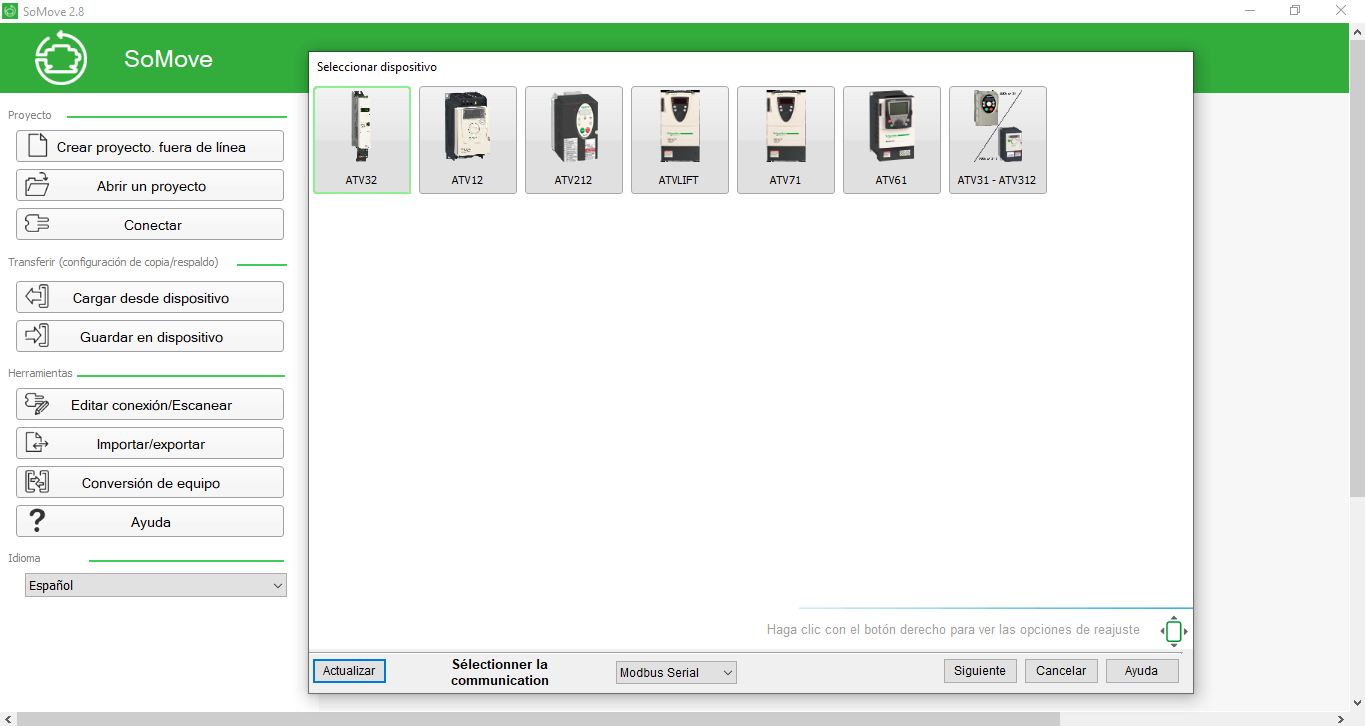
\includegraphics[width=0.9\linewidth]{somove1.png}
	\captionof{figure}{Elección de Altivar 312}
	\label{fig:so1}
\end{figure}
\begin{figure}[H]
	\centering
	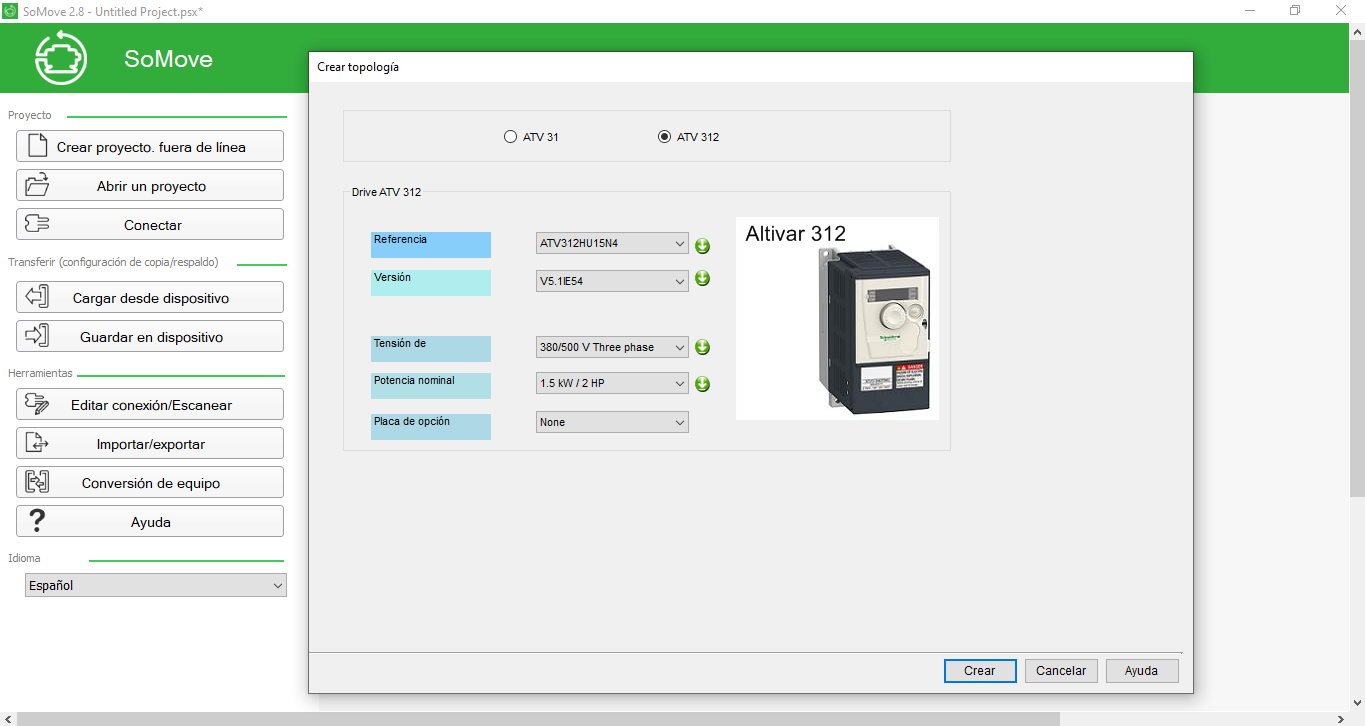
\includegraphics[width=0.9\linewidth]{somove2.png}
	\captionof{figure}{Parámetros del variador}
	\label{fig:so2}
\end{figure}

\begin{figure}[H]
	\centering
	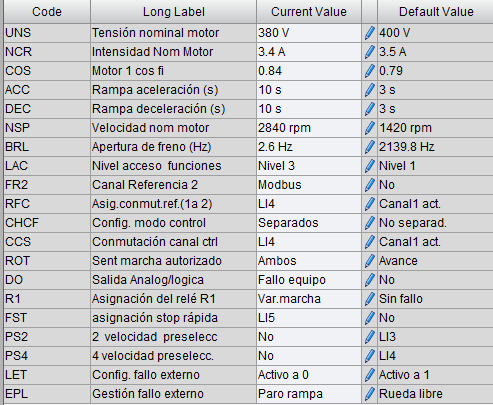
\includegraphics[width=0.7\linewidth]{images/paramsomove}
	\captionof{figure}{Lista de parámetros modificados}
	\label{fig:paramsomove}
\end{figure}


Para realizar esta primera configuración se comunicó la computadora con el variador a través del protocolo \textit{Modbus RTU} (Figura \ref{fig:pcvar}) por medio de un cable RJ45 / par trenzado y un conversor RS485 / USB (Figura \ref{fig:paramsomove1}). 
\begin{figure}[H]
	\centering
	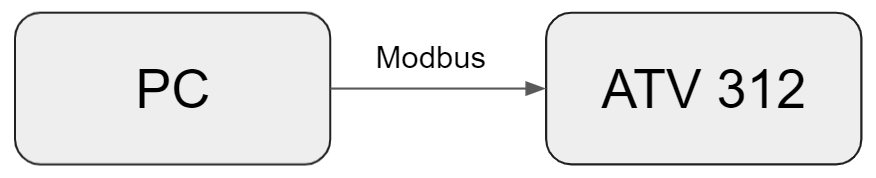
\includegraphics[width=0.7\linewidth]{pc_var.png}
	\captionof{figure}{Diagrama de comunicación PC- variador}
	\label{fig:pcvar}
\end{figure}

\begin{figure}[H]
	\centering
	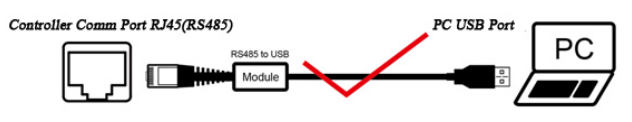
\includegraphics[width=0.9\linewidth]{paramsomove1.png}
	\captionof{figure}{Cable de comunicación}
	\label{fig:paramsomove1}
\end{figure}


\subsection{Comunicación variador de velocidad - PLC}
Para poder realizar la comunicación entre el variador y el PLC fue necesario contar con un cable RJ45 (variador) a DB9 (PLC) a través del protocolo CANopen (Figura \ref{fig:cable}), y se colocó en los finales de línea una resistencia de 120 $\Omega$ para evitar ruidos eléctricos y fenómenos de reflexión en la línea.


\begin{figure}[htbp]
    \centering
    \subfigure[Ficha entrada/salida variador]{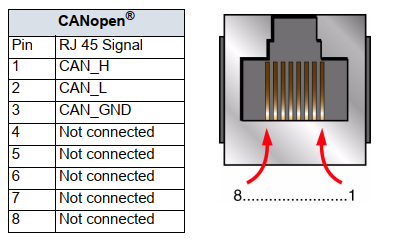
\includegraphics[width=60mm]{canconectores.png}}
    \subfigure[Ficha entrada/salida PLC]{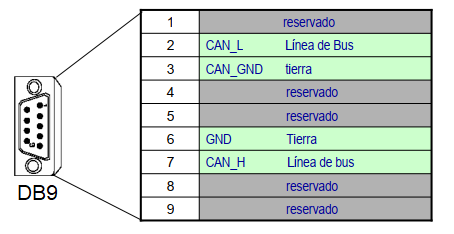
\includegraphics[width=80mm]{candb9.png}}
    \caption{Conexión fichas RJ45- DB9} \label{fig:cable}
    \end{figure}



\subsection{Programación Unity Pro}


Para generar la base del proyecto de trabajo, se descargó e instaló el software \textit{Unity Pro XL} y la librería DTM utilizada en el software \textit{soMove} correspondiente al variador que se posee. Una vez que fue instalado se creó y configuró un nuevo proyecto a través de los siguientes pasos.
\begin{enumerate}
	\item Se seleccionó el bastidor (Figura \ref{fig:uni0}).
	\item En la configuración gráfica del bastidor 
se introdujo los módulos
	deseados (Figura \ref{fig:uni1}) correspondientes al PLC didáctico del laboratorio (Sección \ref{sec:didac}). 
	\item Se configuró el módulo Ethernet, desde el explorador de
	proyectos se desplegó la
	carpeta \textit{Comunicación} y se creó una nueva red, Ethernet (Figura \ref{fig:inter}).
	\item Se añadió en el bus CANopen el variador utilizado (Figura \ref{fig:vcan}). En nuestro caso se eligió el ATV31 para usar los bloques de funciones de control de movimiento preestablecidos por el software. Dentro de las configuraciones de este protocolo se configuró la velocidad de transmisión de este dispositivo. \ref{fig:CAN01}
	\item Se creó una nueva sección de lenguaje FDB para visualizar los parámetros básicos.
	\begin{itemize}
		\item Los \textit{Diagramas de Bloques de Función} consisten en un editor gráfico orientado al dibujo
		de bloques. Este se basa en la utilización de funciones reusables elementales y
		derivados.
	\end{itemize}
%\item Para realizar la conexión del PLC con la computadora se utiliza protocolo TCP/IP a través de la dirección 192.168.10.187 (Dirección que el PLC tiene configurada internamente)(Figura \ref{fig:direcc}) y (Figura \ref{fig:inter})
\end{enumerate}
	
	\begin{comment}
	que posee los siguientes módulos:
\begin{itemize}
\item BMX XBP 0400: bastidor para 4 módulos más la fuente de alimentación.
\item BMX P34 2030: CPU 340-20 Ethernet CANopen.   (Comunicación)
\item BMX ART 0414: 4 entradas TC/RTD con separación de potencial.
\item BMX DDM 16022: 8 entradas digitales, y 8 salidas digitales por transistor PNP, todas ellas aisladas.
\item BMX CPS 2000: Fuente de alimentación de 220V
\end{itemize}

	\end{comment}


\begin{center}
	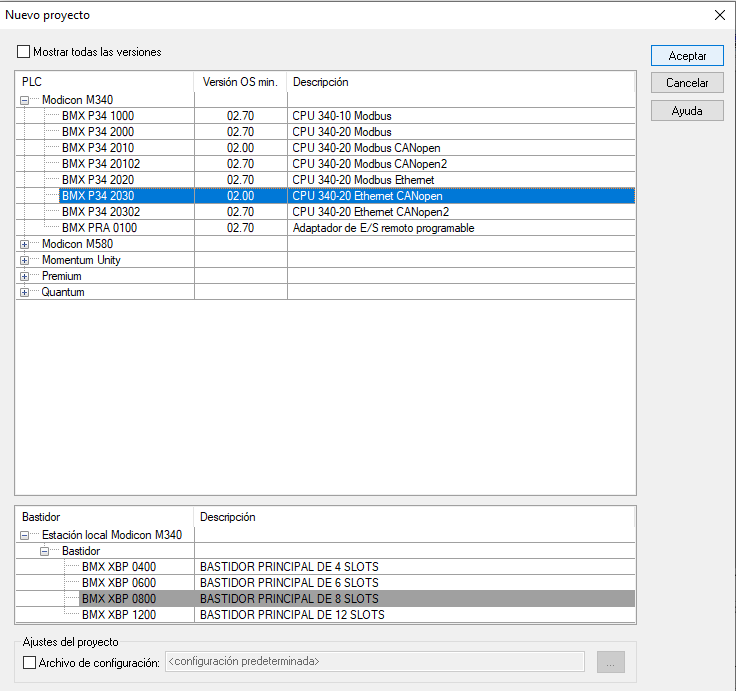
\includegraphics[width=0.8\linewidth]{unit1.png}
	\captionof{figure}{Elección del bastidor}
	\label{fig:uni1}
	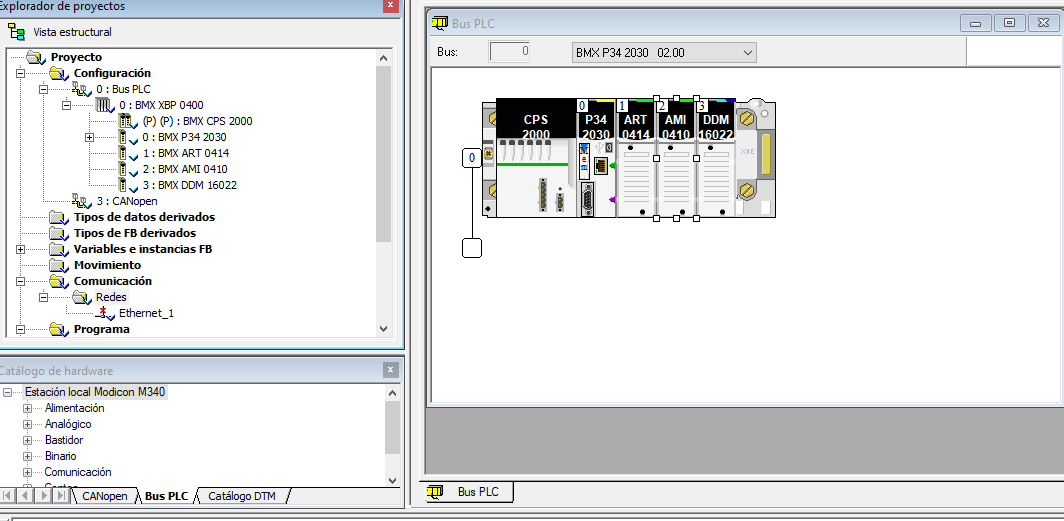
\includegraphics[width=0.8\linewidth]{unity1.png}
	\captionof{figure}{Módulos PLC}
	\label{fig:uni0}
\end{center}

%\begin{figure}[h]
%	\centering
%	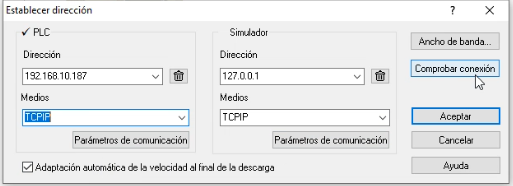
\includegraphics[scale=1]{1.direcc.png}
%	\captionof{figure}{Dirección IP}
%	\label{fig:direcc}
%\end{figure}


\begin{figure}[h]
	\centering
	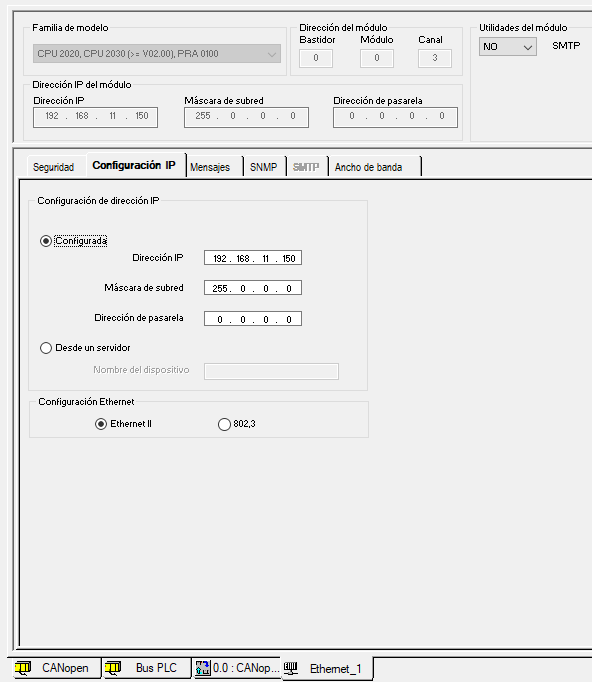
\includegraphics[width=0.8\linewidth]{2.ethern.png}
	\captionof{figure}{Dirección módulo Ethernet}
	\label{fig:inter}
\end{figure}

\begin{figure}[h]
	\centering
	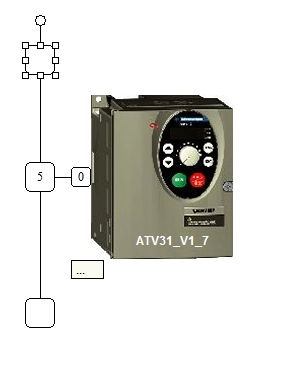
\includegraphics[width=0.6\linewidth]{vcan.png}
	\captionof{figure}{Configuración variador CANopen}
	\label{fig:vcan}
\end{figure}

\begin{figure}[h]
	\centering
	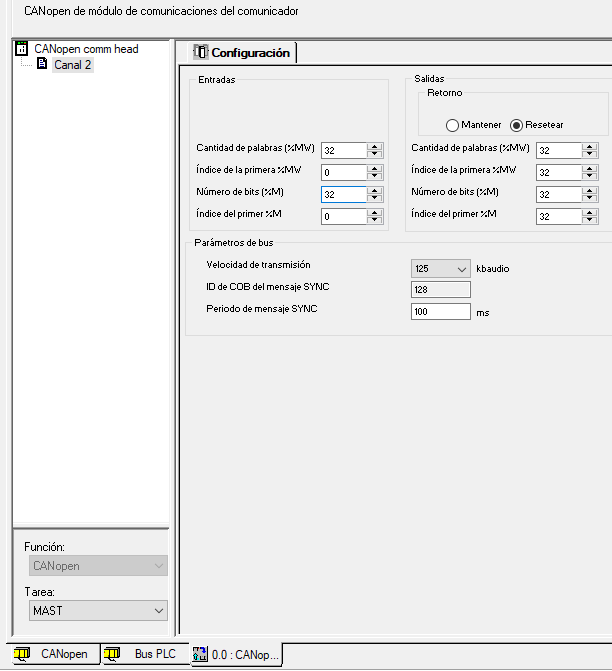
\includegraphics[width=0.8\linewidth]{CAN01.png}
	\captionof{figure}{Configuración variador CANopen}
	\label{fig:CAN01}
\end{figure}

Una vez que se completó la configuración de la comunicación variador - PLC se procedió a crear un HMI simple en\textit{ iFix} (Figura \ref{fig:previo}), el cual fue utilizado para interactuar y observar diversos parámetros, modificar velocidades, observar señales luminosas y ver distintos valores proporcionados por el variador de velocidad.
 
\begin{figure}[H]
	\centering
	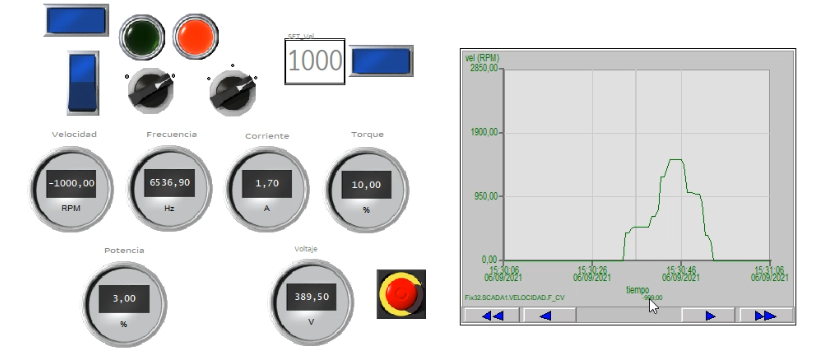
\includegraphics[width=0.9\linewidth]{3.previo.png}
	\captionof{figure}{HMI simple}
	\label{fig:previo}
\end{figure}

Para observar en el HMI se utilizó los MFB del software \textit{UnityPro} (Figura \ref{fig:read}), los cuales necesitan de un bloque maestro ``CAN\_HANDLER'' el cual permite comprobar la comunicación \textit{CANopen}.

Otros de los bloques más utilizados dentro del programa fue ``MC\_READPARAMETER'' que se utiliza para leer, mediante mensajes SDO, una variable del variador definida en una dirección \textit{CANopen} dada por el fabricante \cite{ComManual}.

\begin{figure}[H]
	\centering
	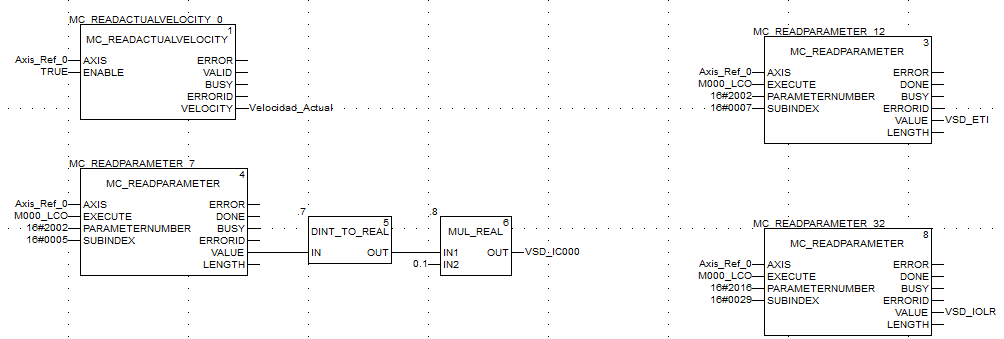
\includegraphics[width=0.9\linewidth]{4.read.png}
	\captionof{figure}{Programa con bloques MFB}
	\label{fig:read}
\end{figure}



\subsubsection{Entradas analógicas}
En el rack del PLC se encuentra un módulo AMI0410 el cual consiste en cuatro entradas analógicas (Tensión/Corriente) aisladas del siguiente tipo:
\begin{itemize}
	\item Corriente +/- 20 mA
\item 	Corriente 0 a 20 mA
\item 	Corriente 4 a 20 mA
\item 	Tensión +/- 10 V
\item 	Tensión +/- 5 V
\item 	Tensión 0 a 10 V
\item 	Tensión 0 a 5 V
\item 	Tensión 1 a 5 V
	
\end{itemize}

El módulo dispone de 20 bornes accesibles al usuario dónde el diagrama de conexión tanto para entradas de tensión o de corriente es el mostrado en la figura \ref{fig:modulo}.

Para realizar la configuración de los transmisores de presión en \textit{Unity PRO} se elige, de las opciones nombradas anteriormente, la que se utilizó en este caso de 4 a 20 mA y el escalado predefinido de fábrica de 0 a 10000 cuentas, pero modificable por el usuario entre -32768 a 32767 ya que la resolución de las entradas analógicas es de 16 bits. También se agregó un filtro de primer orden a cada entrada por software (Figura \ref{fig:param}).

Con el rango de cuentas del módulo determinado, se requirió escalar la variable para obtener el valor físico y así utilizarla para la visualización y control del banco de pruebas.

Para el escalado de la señal de entrada se realizó un nuevo bloque FB derivado, a partir elementos primarios, para evitar realizar un proceso repetitivo en el escalado de varias señales (Figura \ref{fig:escalado}).

En la variable de entrada se coloca la señal que se desea escalar, en los límites de entrada se escribe el rango del módulo visto anteriormente, y en los límites de salida, los escalados obtenidos del instrumento que se utilizó.

 Finalmente, a la salida del bloque se obtuvo el valor físico visualizado o transmitido por el instrumento.

\begin{figure}[H]
	\centering
	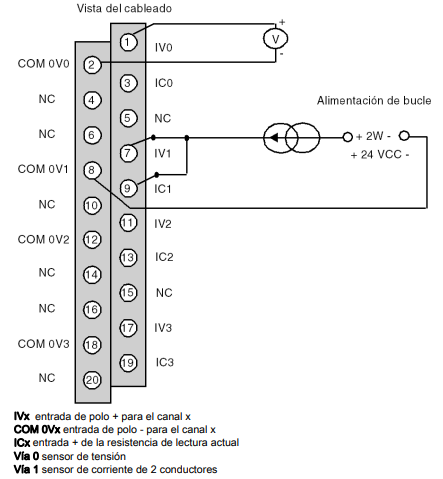
\includegraphics[width=0.6\linewidth]{modulo.png}
	\captionof{figure}{Módulo AMI0410}
	\label{fig:modulo}
\end{figure}

\begin{figure}[htbp]
	\centering
	\subfigure[]{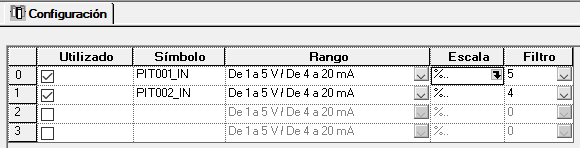
\includegraphics[scale=0.8]{parama.png}}
	\subfigure[]{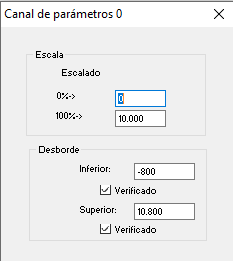
\includegraphics[scale=1]{param.png}}
	\caption{Rango y escalado} \label{fig:param}
\end{figure}




\begin{figure}[H]
	\centering
	\subfigure[]{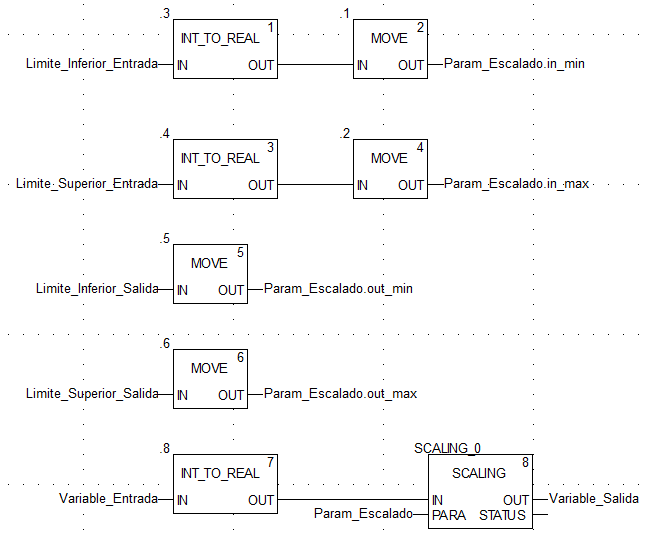
\includegraphics[scale=0.5]{escalado01.png}}
	\subfigure[]{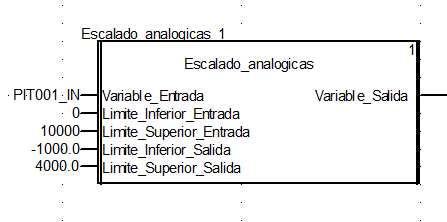
\includegraphics[scale=0.5]{escalado02.png}}
	\caption{Bloques de escalado}
	\label{fig:escalado}
\end{figure}


\subsubsection{Entradas analógicas para termocuplas o RTD}
Se utilizó el módulo ART0414 que consiste en cuatro entradas aisladas en las que se puede conectar sensores de temperatura del tipo termocupla y RTD con las siguientes características:
\begin{itemize}
	\item RTD IEC Pt100/Pt1000, US/JIS Pt100/Pt1000, Cu10, Cu50, Cu100, Ni100/Ni1000 en 2, 3 o 4 conductores
	\item Termoelemento del tipo B, E, J, K, L, N, R, S, T, U
\item 	Tensión $+/-$ 40 mV a 1,28 V
	
\end{itemize}

Para la conexión de estos sensores se utiliza el accesorio TELEFAST ABE-7CPA412 (Figura \ref{fig:ABE}) y según el tipo de sensor se tiene las conexiones que se muestran en la figura \ref{fig:ABE2}.

\begin{figure}[H]
	\centering
	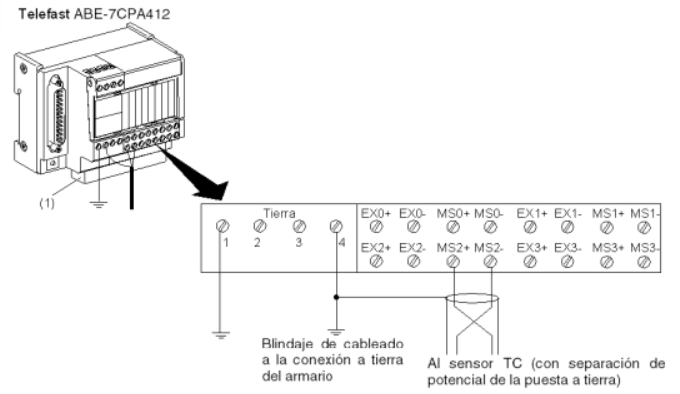
\includegraphics[width=0.9\linewidth]{ABE.png}
	\captionof{figure}{Accesorio TELEFAST ABE-7CPA412}
	\label{fig:ABE}
\end{figure}
\begin{figure}[H]
	\centering
	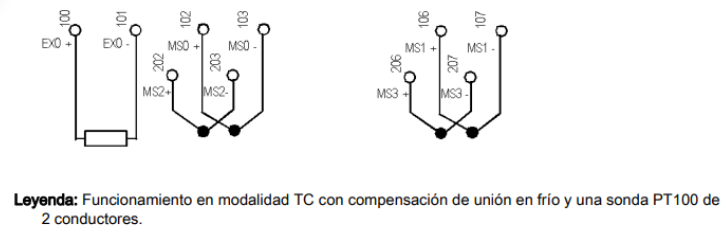
\includegraphics[width=0.9\linewidth]{ABE2.png}
	\captionof{figure}{Tipos de conexión}
	\label{fig:ABE2}
\end{figure}

Para configurar en \textit{Unity Pro} se seleccionó en \textit{rango} la característica resistiva del sensor. En el caso de RTD y termocupla los valores de salida son múltiplos de 10 de la temperatura. 

En la imagen \ref{fig:ABE3} se observa dos elementos ya que se probó realizar la configuración con una termocupla y un RTD. Finalmente se eligió el RTD PT1000 ya que dispone de una superficie plana que mejora el contacto con la carcasa del motor. El valor obtenido a la salida del módulo se divide por 10 y se genera el valor de temperatura en °C con un decimal  (Figura \ref{fig:ABE3}).

\begin{figure}[H]
	\centering
	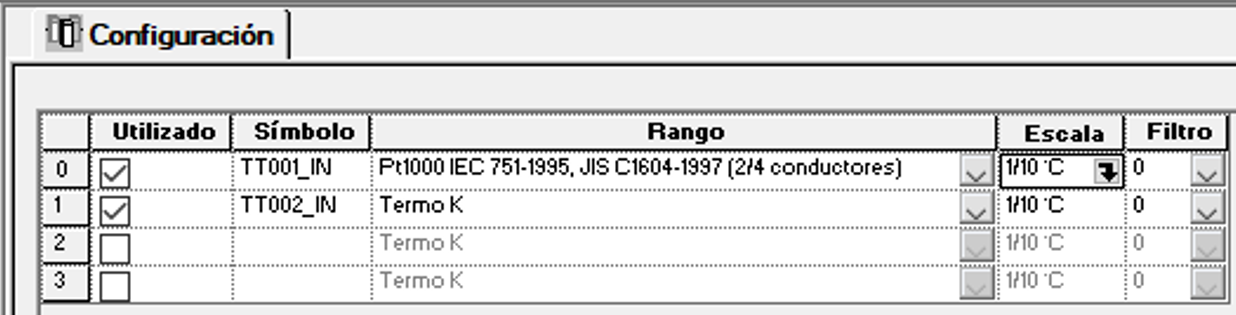
\includegraphics[width=0.9\linewidth]{ABE3.png}
	\captionof{figure}{Rango y escalado}
	\label{fig:ABE3}
\end{figure}

\begin{figure}[H]
	\centering
	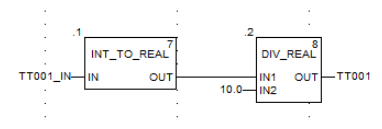
\includegraphics[width=0.6\linewidth]{ABE4.png}
	\captionof{figure}{Bloque de escalado}
	\label{fig:ABE4}
\end{figure}

\subsubsection{Medición de caudal}
A la salida del caudalímetro se obtiene pulsos con frecuencia proporcional al flujo. Para ser procesados por el PLC se utilizó un módulo externo al PLC por la baja tasa de refresco que posee el módulo de entradas digitales. Para esto se planteó utilizar un ESP8266 como interfaz para obtener los pulsos, colocarlos en un registro y enviarlos por un servidor Modbus TCP cada 20ms al PLC. En la sección de programación del PLC se realizó las cuentas correspondientes para generar la conversión de pulsos a caudal (Figura \ref{fig:modtcp}). El módulo y el caudalímetro alimentó mediante una fuente externa de 3,3 V.
\begin{figure}[htbp]
	\centering
	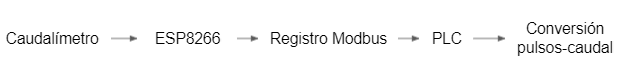
\includegraphics[scale=1]{esp_mod.png}
	\captionof{figure}{Diagrama de flujo del caudalimetro} 
	\label{fig:modtcp}
\end{figure}
\newpage

%\url{
%https://download.schneider-electric.com/files?p_enDocType=User+guide&p_File_Name=35010608_K01_000_11.pdf&p_Doc_Ref=35010608K01000}
